\newpage
\section{Proposed solution} \label{solution}

In this section we propose the approaches with centralized coordination.
In a warehouse the connection between robots is efficient and has no big limitations.
\begin{enumerate}
  \item The first strategy, mentioned above, is the \srst which consider only 
  one task allocated for one robot.

  \item The second strategy \sps using an optimal approach
  to compose tasks. Precisely resolve the set partition problem of set tasks $\mathcal{T}$ . 
  
  \item The last strategy (\gsp) extends the first algorithm,
  the main concept of this strategy is composing the tasks in a single travel with greedy coalition formation approach. 
  
\end{enumerate}

In section \ref{chap:conclusions} as a future development we want to explore a distributed 
method because in this thesis we  only focused in centralized method.  

\subsection{Single robot : Single task (\srst)}

This method is a baseline for our logistic scenario.
The important constraint of this approach is to consider only one task allocated for 
one robot at time.
\\
The set of tasks is ordered by the function mentioned below.
\begin{algorithm}
  \caption{Pop minimum element} \label{SP}
  \begin{algorithmic}[1]
    
    \Procedure{PME}{$T_i, T_j \in \mathcal{T}$}
    \If{$(demand(T_i) < demand(T_j)) \wedge (dst(T_i) < dst(T_j))$}
    \State {\bf return} true
    \Else
    \If{$dst(T_i) = dst(T_j)$}
    \State {\bf return} true
    \EndIf
    \State {\bf return} false
    \EndIf
    \EndProcedure
  \end{algorithmic}
\end{algorithm}
\newpage
Such function sorts the tasks based on the distance of the unloading bays and the demand of a specific task.
For distance we consider the euclidean distance between loading bay $L$ and unloading bays $U_j$.
Instead for demand is the weight of the item.

After the choose of the task to allocate by using the function $f(P)$ return the path distance, precisely the cost of the trail.

For this method we do not use the function $p(\cdot)$ because we have only one task for robot
then the task already has the path. As mentioned above, we do not combine routes.

For completeness in this method we do not consider the heuristic function $v(\cdot)$ because the demand for all
task is always 1. Because we allocate only one task for one robot at time.

This algorithm take linear time or $O(n)$ time, its time complexity is $O(n)$.
This means that the running time increases at most linearly with the size of the input.
More precisely, this means that there is a constant $c$ such that the running time is 
at most $cn$ for every input of size $n$.



\begin{figure} [hbt]
  \centering
  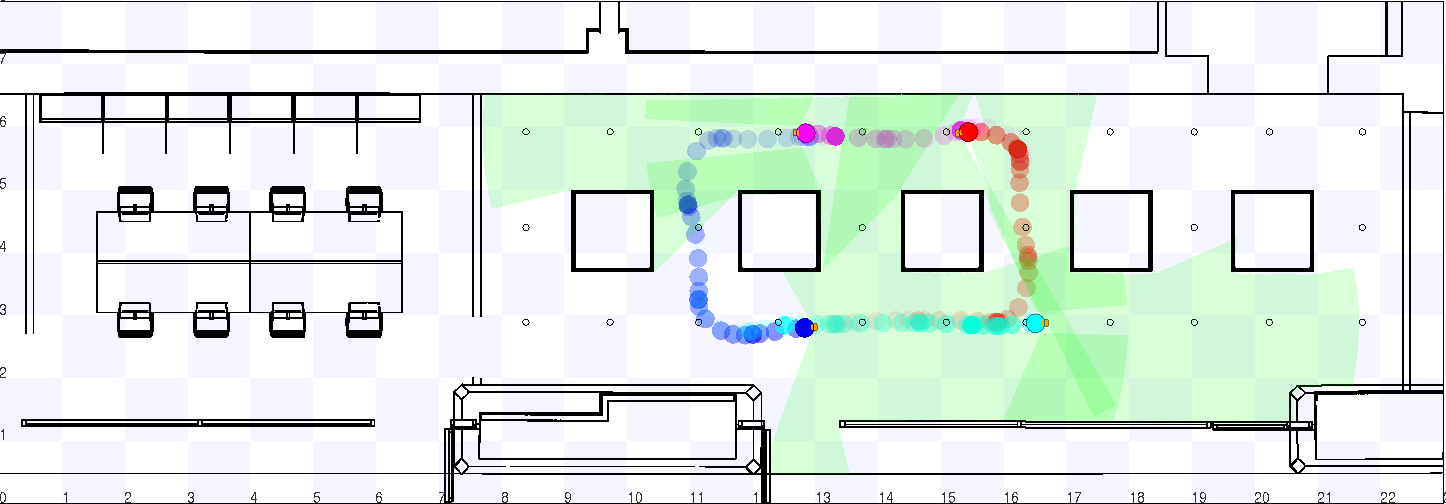
\includegraphics[width=\textwidth]{img/cycle1.png}
  \caption{Example of execution \srst with 4 agents with capacity 4 and 9 tasks.}
  \label{fig:srst}
\end{figure}



\subsection{Set Partition Strategy - Single robot : Multiple task (\sps)}

This method consists to compute all possible patitions of the task set 
using Set Partition algorithm \cite{partition} and use only 
the best partition which is based on the previously mentioned heuristic $v(\cdot)$.

After initialzation phase which all agents send their capacity and identifier,
start the partition algorithm \cite{partition} that return all possible patitions of subsets combination 
of tasks $P^N$.

Then foreach partitions the heuristic $v(\cdot)$ has been used to calculate the loss.
For calculate the loss $L$ of a partition we have to calculate the $v(\cdot)$ for all elements in
the subsets partition and finally sum all values for all subsets. 
Furthermore the combination with the lowest loss has been choose.
So a subset of combination as been sort in a increasing order. 
Then the first subset of combination has the lowest value of heuristic function 
is the first task assigned at the first request from a robot.

\begin{algorithm}
  \caption{Set Partition Strategy} \label{SP}
  \begin{algorithmic}[1]
  \Procedure{SPS}{$P^N$}\Comment{$P^N$= \texttt{partition(}$\mathcal{T}$\texttt{)}}
  \State \Comment{define $C$ the maximum capacity of the robots}
  \For{$P_i \in P^N$}
  \If{$demand(P_i) > C$}
  $P^N \setminus P_i$
  \EndIf
    \For{$S_j \in P_i$}
      $v(S_j)$ 
    \EndFor
  \EndFor
  \Comment{sort all $P_i$ for lowest $v(\cdot)$} 
  \State {\bf return} the first $P_i$
  \EndProcedure
  \end{algorithmic}
\end{algorithm}

The function \texttt{partition($\cdot$)} take exponential time. 

More formally, this algorithm is exponential time because $T(n)$ is bounded by $O(2^{n^{k}})$ 
for some constant $k$.

\newpage

An example of solution with set $|\mathcal{T}| = 4$:
\begin{center}
  \begin{tabular}{|c|r|c|} \hline
  \textbf{iteration} & \textbf{partition size} & \textbf{partition} \\ \hline
  1    & 1    & \{\{a, b, c, d\}\}   \\
  2    & 2    & \{\{a, b, c\}, \{d\}\}   \\
  3    & 2    & \{\{a, b, d\}, \{c\}\}   \\
  4    & 2    & \{\{a, b\}, \{c, d\}\}   \\
  5    & 3    & \{\{a, b\}, \{c\}, \{d\}\}   \\
  6    & 2    & \{\{a, c, d\}, \{b\}\}   \\
  7    & 2    & \{\{a, c\}, \{b, d\}\}   \\
  8    & 3    & \{\{a, c\}, \{b\},\{d\}\}   \\
  9    & 2    & \{\{a, d\}, \{b, c\}\}   \\
  10   & 2    & \{\{a\}, \{b, c, d\}\}   \\
  11   & 3    & \{\{a\}, \{b, c\}, \{d\}\}   \\
  12   & 3    & \{\{a, d\}, \{b\}, \{c\}\}   \\
  13   & 3    & \{\{a\}, \{b, d\}, \{c\}\}   \\
  14   & 3    & \{\{a\}, \{b\}, \{c, d\}\}   \\
  15   & 4    & \{\{a\}, \{b\}, \{c\},\{d\}\}   \\ \hline       
  \end{tabular}
\end{center}



For $|\mathcal{T}| = 4$ takes 0.000043 seconds. If we increase the set, time increases exponentially.
An example of $|\mathcal{T}| = 12$ takes 2.8 seconds and $|\mathcal{T}| = 13$ takes 21.2 seconds.

For this reason in our experiment we limited the size of the task set at most 9 tasks.

\begin{figure} [hbt]
  \centering
  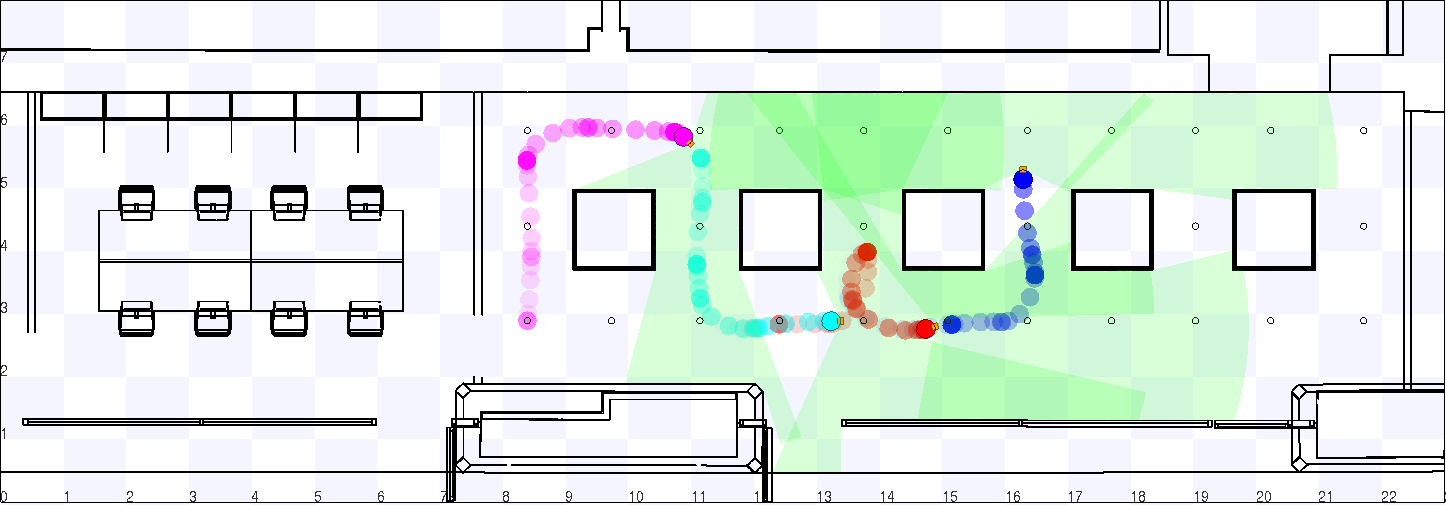
\includegraphics[width=\textwidth]{img/opt.png}
  \caption{Example of execution \sps with 4 agents with capacity 4 and 9 tasks. See example \ref{example}}
  \label{fig:srst}
\end{figure}

\subsection{Greedy Set Partition Strategy - Single robot : Multiple task (\gsp)}
The main concept of this approach is composing tasks using Greedy Coalition Formation
based on \cite{cf_greedy} and \cite{cf_farinelli}. Where one wants to minimize the 
team cost subject to the constraint that each task must be executed by a given 
number of cooperative agents simultaneosly. Each task requires a number of different 
demands, and each coalition for the task needs to provide the requered capabilities.

Later initialzation phase which all agents send their capacity and identifier,
start the Coalition Formation algorithm \cite{cf_greedy}.
When compute new one possible coalition the heuristic  $v(\cdot)$ has been used to calculate 
the loss $L(T_{i,j})$ and if is negative that coalition is insered into the formation and the 
$T_i$ , $T_j$ are deleted from the task set $\mathcal{T}$.

\begin{algorithm}
\caption{Greedy Coalition Formation} \label{GCF}
\begin{algorithmic}[1]
  \Procedure{GCF}{$\mathcal{T}$}\Comment{$\mathcal{T}$ = set of tasks}
  \State \Comment{define $C$ the maximum capacity of the robots}
  \For{$T_i \in \mathcal{T}$}
  \For{$T_j \in \mathcal{T}$}
\Comment{define $T_{i,j} = T_i \cup T_j$}
\If{$(T_i \neq T_j) \wedge (demand(T_{i,j}) \leq C)$}
\If{$v(T_{i,j})-v(T_i)-v(T_j) < 0$}
       \State $\mathcal{T} \setminus \{ T_i\} \setminus \{T_j\}$ $\mathcal{T} \cup \{T_{i,j}\}$
  \EndIf
  \EndIf
\EndFor
\EndFor
\State {\bf return} $\mathcal{T}$
\EndProcedure
\end{algorithmic}
\end{algorithm}

This algorithm take polynomial time, its running time is upper bounded by a polynomial expression
in the size of the input for the algorithm.

More precisely, this algorithm take $O(n^k)$ for some positive constant $k$. 

\begin{figure} [hbt]
  \centering
  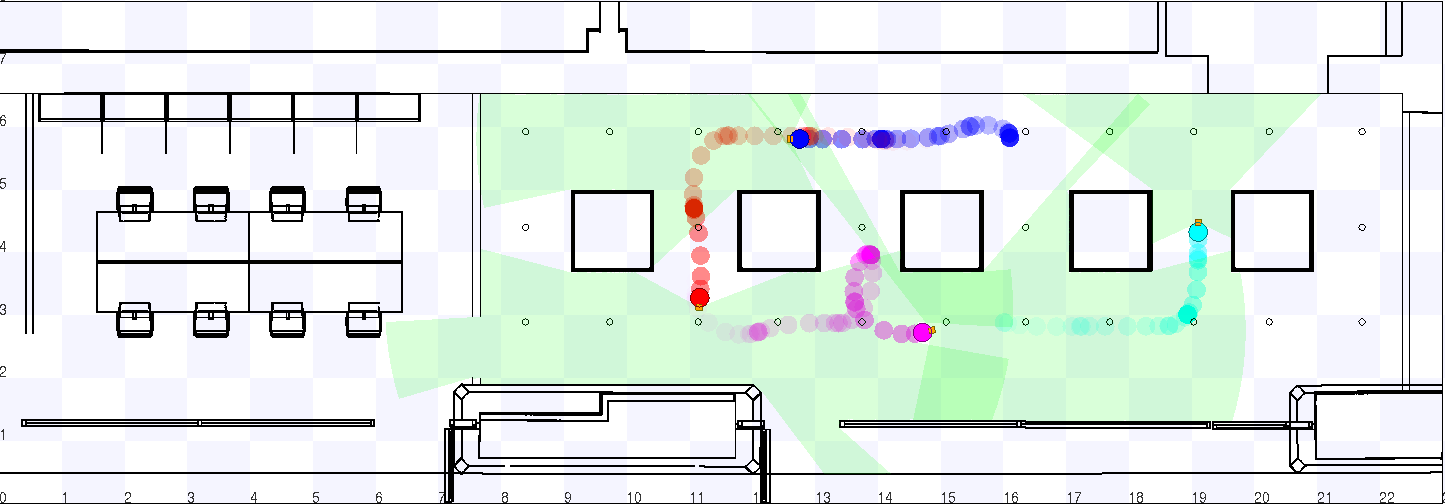
\includegraphics[width=\textwidth]{img/cf.png}
  \caption{Example of execution \gsp with 4 agents with capacity 4 and 9 tasks. See example \ref{example}}
  \label{fig:srst}
\end{figure}


\newpage
\subsection*{Example with 9 tasks and 4 robots} \label{example}
Given a set of tasks $\mathcal{T}= \{  \{T_0\}, \{T_1\}, \cdots, \{T_8\} \}$ defined like:

${T_i=(item, demand, unloading\_bay)}$.

The agents have the same capacity $C_{0,1,2,3} = 4$.
\begin{table}[hbt]
\begin{center}
  % \centering
  \begin{tabular}{|c|c|c|c|} \hline
    \textbf{task} & \textbf{item} & \textbf{demand} & \textbf{unloading bay} \\ \hline
    0    & A    & 1      & 0             \\
    1    & B    & 2      & 1             \\
    2    & C    & 3      & 2             \\
    3    & A    & 1      & 0             \\
    4    & B    & 2      & 1             \\
    5    & C    & 3      & 2             \\
    6    & A    & 1      & 0             \\
    7    & B    & 2      & 1             \\
    8    & C    & 3      & 2             \\ \hline       
  \end{tabular}
  \caption{The task set $\mathcal{T}$ for 9 tasks}
  \label{tab:t4} 
\end{center}
\end{table}

Given a finite task set $\mathcal{T}$ we can see how our strategies works.
For this example we have created a video of the simulations execution, in ROS and stage, which are available on YouTube \footnote{YouTube site https://youtu.be/XbdBklu98HE}.
\newpage
The \sps created 5 orders to perform all elements in the tasks set.

In the table \ref{tab:sps} we can see the partition composed by subsets of tasks.
\begin{table}[hbt]
  \begin{center}
    \begin{tabular}{|c|c|c|c|} \hline
    \textbf{task} & \textbf{item} & \textbf{demand} & \textbf{unloading bay} \\ \hline
    \{4,7\}    & B    & 4     & \{1\}             \\
    \{0,1,3\}  & \{A,B\}& 4    & \{0,1\}             \\
    \{2,6\}    & \{C,A\}    & 4  & \{0,2\}             \\
    5    & C    & 3      & 2             \\
    8    & C    & 3      & 2             \\ \hline       
    \end{tabular}
    \caption{The result of the Set Partition Strategy (\sps)}
    \label{tab:sps}
  \end{center}
\end{table}

The \gsp creted 6 orders, one more than \sps, to perform all elements in the tasks set.

In table \ref{tab:gsp} we can see the partition composed by subsets of tasks.
\begin{table}[hbt]
\begin{center}
  \begin{tabular}{|c|c|c|c|} \hline
  \textbf{task} & \textbf{item} & \textbf{demand} & \textbf{unloading bay} \\ \hline
  \{3,2\}    & \{A,C\}    & 4     & \{0,2\}             \\
  \{0,1\}    & \{A,B\}    & 3     & \{0,1\}             \\
  \{6,4\}    & \{A,B\}    & 3     & \{0,1\}             \\
  5    & C    & 3      & 2             \\
  8    & C    & 3      & 2             \\        
  7    & B    & 2      & 1             \\\hline
  \end{tabular}
  \caption{The result of the Greedy Set Partition (\gsp)}
  \label{tab:gsp}
\end{center}
\end{table}

\newpage
In this Figure \ref{fig:CF_graph} we can see because the Greedy approach is less
complex than \sps. On the execution before to create a coalition is checked if its can 
be allocated. This check is the value of the loss of the coalition, if is less than zero
the colaition is insered in the solution else break the cycle for and pass another coalition.  

\begin{figure} [hbt]
    \centering
    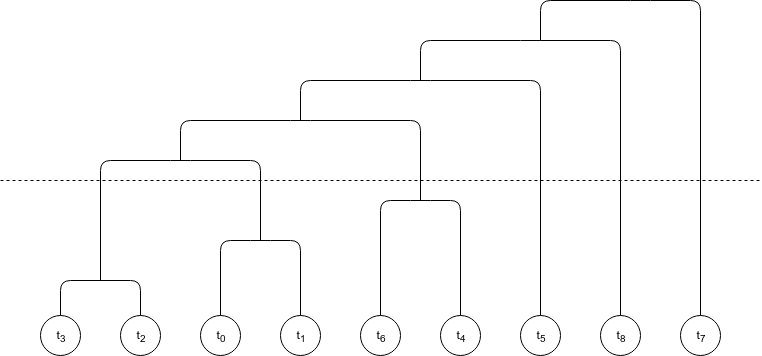
\includegraphics[width=\textwidth]{img/CF.png}
    \caption{The horizontal line represents a cut on executin defines the coalition structure.}
    \label{fig:CF_graph}
\end{figure}

